% Generated on 2023-10-27 10:45:21 by gEcon ver. 1.2.1 (2023-01-18)
% http://gecon.r-forge.r-project.org/

% Model name: RW

\section{Steady-state values}


\begin{tabular}{c|c|}
  & Steady-state value\\
\hline
${e\!t\!a\!p\!i}$ & 1 \\
$i$ & 0 \\
$\lambda^{\mathrm{RW}^{\mathrm{1}}}$ & -0.683 \\
$\lambda^{\mathrm{RW}^{\mathrm{2}}}$ & 0 \\
$\pi$ & 0 \\
$y$ & -4.0568 \\
$U$ & -33.8066 \\
\hline
\end{tabular}


\section{The solution of the 1st order perturbation}

\subsection*{Matrix $P$}

$$\bordermatrix{
~ & {e\!t\!a\!p\!i}_{t-1} & i_{t-1} & \pi_{t-1} & y_{t-1} \cr
{e\!t\!a\!p\!i}_{t} & 0.95 & 0 & 0 & 0 \cr
i_{t} & -13.033 & -1.9422 & 5.8225 & -13.7015 \cr
\pi_{t} & -1.0101 & 0 & 1.0101 & -1.0101 \cr
y_{t} & 0.249 & 0.2465 & -0.249 & 1.249 \cr
}$$

\subsection*{Matrix $Q$}

$$\bordermatrix{
~ & \epsilon^{\pi} \cr
{e\!t\!a\!p\!i} & 1 \cr
i & -7.59 \cr
\pi & 0 \cr
y & 0 \cr
}$$

\subsection*{Matrix $R$}

$$\bordermatrix{
~ & {e\!t\!a\!p\!i}_{t-1} & i_{t-1} & \pi_{t-1} & y_{t-1} \cr
\lambda^{\mathrm{RW}^{\mathrm{1}}}_{t} & -8.6776 & -0.7328 & 4.9879 & -7.9606 \cr
\lambda^{\mathrm{RW}^{\mathrm{2}}}_{t} & 0.9938 & 0.1309 & -0.5005 & 1.0316 \cr
U_{t} & -0.3395 & 0 & 0.0202 & -0.0202 \cr
}$$

\subsection*{Matrix $S$}

$$\bordermatrix{
~ & \epsilon^{\pi} \cr
\lambda^{\mathrm{RW}^{\mathrm{1}}} & -3.8839 \cr
\lambda^{\mathrm{RW}^{\mathrm{2}}} & 0.5193 \cr
U & -0.3361 \cr
}$$


\section{Model statistics}

\subsection{Basic statistics}

\begin{tabular}{c|c|c|c|c|}
  & Steady-state value & Std. dev. & Variance & Loglin\\
\hline
${e\!t\!a\!p\!i}$ & 1 & 0.1303 & 0.017 & Y    \\
$i$ & 0 & 0.7719 & 0.5958 & N    \\
$\lambda^{\mathrm{RW}^{\mathrm{1}}}$ & -0.683 & 0.4292 & 0.1842 & Y    \\
$\lambda^{\mathrm{RW}^{\mathrm{2}}}$ & 0 & 0.0501 & 0.0025 & N    \\
$\pi$ & 0 & 0.0985 & 0.0097 & N    \\
$y$ & -4.0568 & 0.1707 & 0.0292 & Y    \\
$U$ & -33.8066 & 0.0448 & 0.002 & Y    \\
\hline
\end{tabular}


\subsection{Correlation matrix}

\begin{tabular}{c|ccccccc|}
  & ${e\!t\!a\!p\!i}$ & $i$ & $\lambda^{\mathrm{RW}^{\mathrm{1}}}$ & $\lambda^{\mathrm{RW}^{\mathrm{2}}}$ & $\pi$ & $y$ & $U$\\
\hline
${e\!t\!a\!p\!i}$ & 1 & -0.301 & -0.825 & 0.436 & -0.491 & -0.7 & -0.999 \\
$i$ &  & 1 & 0.567 & -0.977 & -0.323 & -0.443 & 0.28 \\
$\lambda^{\mathrm{RW}^{\mathrm{1}}}$ &  &  & 1 & -0.725 & 0.567 & 0.44 & 0.832 \\
$\lambda^{\mathrm{RW}^{\mathrm{2}}}$ &  &  &  & 1 & 0.116 & 0.273 & -0.421 \\
$\pi$ &  &  &  &  & 1 & 0.826 & 0.524 \\
$y$ &  &  &  &  &  & 1 & 0.721 \\
$U$ &  &  &  &  &  &  & 1 \\
\hline
\end{tabular}


\subsection{Cross correlations with the reference variable ($i$)}

\begin{tabular}{c|c|c|c|c|c|c|c|c|c|c|c|c|}
  & $\sigma[\cdot]$ rel. to $\sigma[i]$ & $i_{t-5}$ & $i_{t-4}$ & $i_{t-3}$ & $i_{t-2}$ & $i_{t-1}$ & $i_{t}$ & $i_{t+1}$ & $i_{t+2}$ & $i_{t+3}$ & $i_{t+4}$ & $i_{t+5}$\\
\hline
${e\!t\!a\!p\!i}_{t}$ & 0.169 & 0.098 & 0.131 & 0.177 & 0.258 & 0.444 & -0.301 & -0.254 & -0.21 & -0.169 & -0.132 & -0.099 \\
$i_{t}$ & 1 & -0.028 & -0.035 & -0.051 & -0.093 & -0.219 & 1 & -0.219 & -0.093 & -0.051 & -0.035 & -0.028 \\
$\lambda^{\mathrm{RW}^{\mathrm{1}}}_{t}$ & 0.556 & -0.078 & -0.1 & -0.134 & -0.204 & -0.385 & 0.567 & 0.47 & 0.151 & 0.043 & 0.003 & -0.013 \\
$\lambda^{\mathrm{RW}^{\mathrm{2}}}_{t}$ & 0.065 & 0.04 & 0.051 & 0.071 & 0.122 & 0.269 & -0.977 & 0.043 & 0.043 & 0.041 & 0.038 & 0.035 \\
$\pi_{t}$ & 0.128 & -0.046 & -0.056 & -0.071 & -0.096 & -0.156 & -0.323 & 0.852 & 0.236 & 0.04 & -0.022 & -0.04 \\
$y_{t}$ & 0.221 & -0.069 & -0.092 & -0.121 & -0.164 & -0.245 & -0.443 & 0.551 & 0.273 & 0.164 & 0.111 & 0.078 \\
$U_{t}$ & 0.058 & -0.098 & -0.13 & -0.176 & -0.257 & -0.441 & 0.28 & 0.286 & 0.215 & 0.167 & 0.128 & 0.095 \\
\hline
\end{tabular}


\subsection{Autocorrelations}

\begin{tabular}{c|ccccc|}
  & Lag 1 & Lag 2 & Lag 3 & Lag 4 & Lag 5\\
\hline
${e\!t\!a\!p\!i}$ & 0.713 & 0.471 & 0.271 & 0.11 & -0.016 \\
$i$ & -0.219 & -0.093 & -0.051 & -0.035 & -0.028 \\
$\lambda^{\mathrm{RW}^{\mathrm{1}}}$ & 0.51 & 0.081 & -0.065 & -0.117 & -0.134 \\
$\lambda^{\mathrm{RW}^{\mathrm{2}}}$ & -0.074 & -0.071 & -0.066 & -0.06 & -0.054 \\
$\pi$ & 0.22 & -0.024 & -0.095 & -0.11 & -0.107 \\
$y$ & 0.504 & 0.261 & 0.116 & 0.017 & -0.055 \\
$U$ & 0.725 & 0.459 & 0.256 & 0.097 & -0.025 \\
\hline
\end{tabular}



\pagebreak

\section{Impulse response functions}

\begin{figure}[h]
\centering
\begin{minipage}{0.5\textwidth}
\vspace*{-3em}
\centering
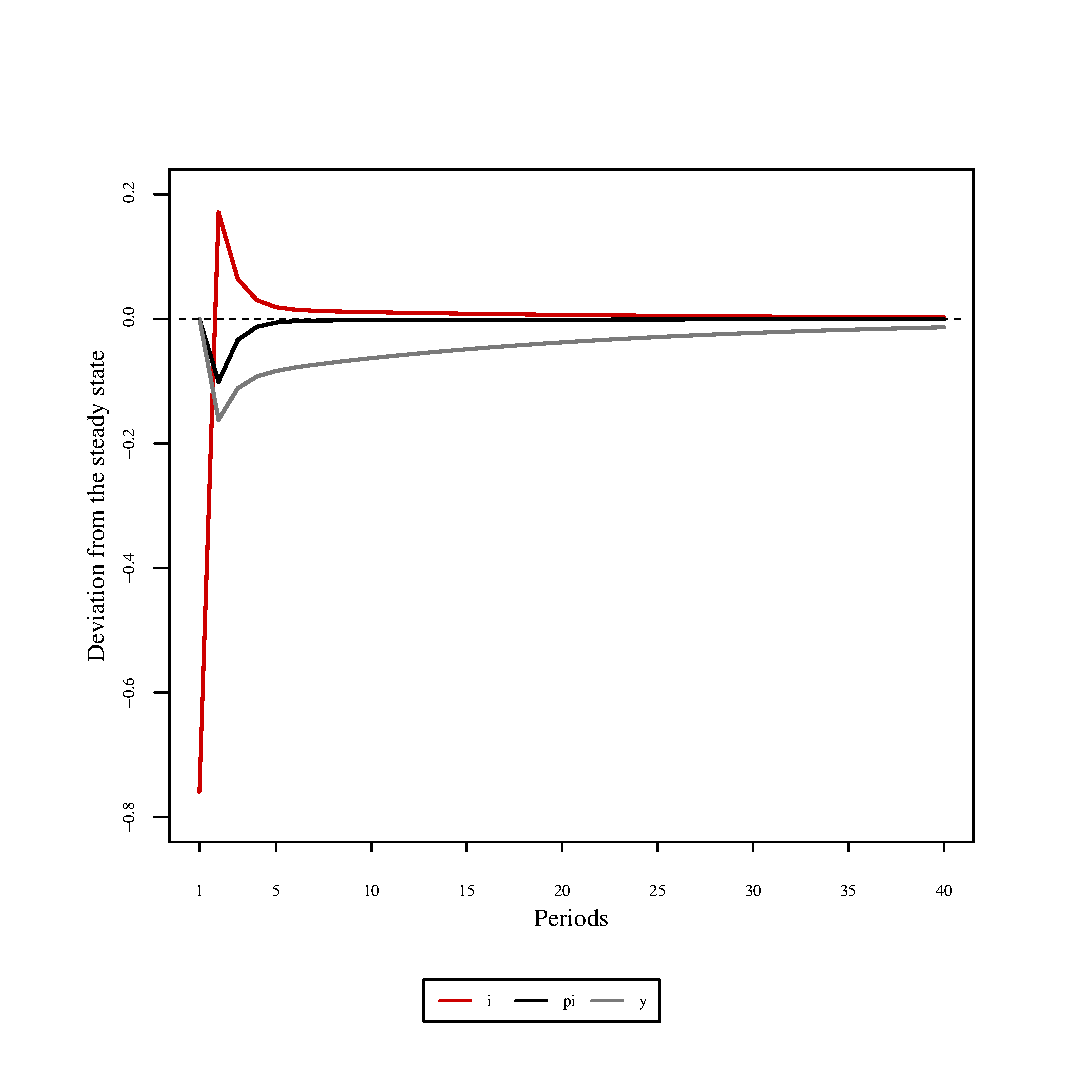
\includegraphics[width=0.99\textwidth, scale=0.55]{plots/plot_21.eps}
\caption{Impulse responses ($i, \pi, y$) to $\epsilon^{\pi}$ shock}
\end{minipage}
\end{figure}
